\documentclass[10pt,a4paper]{amsart}
\usepackage[margin=19mm]{geometry}
\usepackage{amsmath,amssymb,mathtools}
\usepackage[scr=rsfs,cal=euler]{mathalfa}
\usepackage{xfrac}
\usepackage[unicode,hidelinks,bookmarks=false]{hyperref}
\newcommand{\ie}{i.e.\ }
\newcommand{\cf}{cf.\ }
\newcommand{\resp}{respectively\ }
\newcommand{\Subsection}{\subsection}
\providecommand{\nobreakdash}{\nobreak\hbox{-}}
\setlength{\emergencystretch}{2em}
\multlinegap0pt
\usepackage{mathtools}
\usepackage{tikz}
\usetikzlibrary{arrows.meta,positioning,fit,backgrounds,calc,decorations.pathreplacing,calligraphy}
\usepackage{bm}
\usepackage{enumitem}
\usepackage{booktabs}
\newcommand{\R}{\mathbb{R}}
\newcommand{\N}{\mathbb{N}}
\newcommand{\Linf}{L^\infty}
\newcommand{\Lip}{\mathrm{Lip}}
\newcommand{\Tcal}{\mathcal{T}}
\newcommand{\Lipk}{\mathrm{Lip}_K}
\newcommand{\LipT}{\mathrm{Lip}_{\Tcal^{-1}}}
\newcommand{\eps}{\varepsilon}
\newtheorem{theorem}{Theorem}
\newtheorem{lemma}{Lemma}
\newtheorem{proposition}{Proposition}
\newtheorem{definition}{Definition}
\newtheorem{assumption}{Assumption}
\newtheorem{remark}{Remark}
\setlength{\emergencystretch}{5em}
\setlength\abovedisplayskip{.1pt}
\setlength\belowdisplayskip{.1pt}
\setlength\abovedisplayshortskip{.1pt}
\setlength\belowdisplayshortskip{.1pt}
\allowdisplaybreaks
\setlength{\parindent}{2em}
\setlength{\parskip}{0.43em}
\begin{document}
\title[Approximate Feedback Linearization for a Nonlinear Hyperboli]{Approximate Feedback Linearization for a Nonlinear Hyperbolic PDE Class -- Part II: Neural Operator}
\author{Miroslav Krstic}
\date{}
\maketitle
\noindent\emph{Source and licence.} Approximate Feedback Linearization for a Nonlinear Hyperbolic PDE Class -- Part II: Neural Operator. Version arXiv:2607.04362v1 (CC BY 4.0). This material is distributed under the Creative Commons Attribution 4.0 International licence, http://creativecommons.org/licenses/by/4.0/, as recorded in the arXiv OAI licence metadata for this exact version and shown on the abstract page https://arxiv.org/abs/2607.04362v1. Full rights notice: licenses/arxiv-2607.04362-CC-BY-4.0.txt.\par\smallskip
\noindent\textit{Editorial scope.} Counted unit: the original \texttt{theorem} environment \texttt{thm:NO} at source lines 480--488 together with its complete proof at lines 490--492; the delivered document keeps source lines 126--493 so that every referenced label and every citation resolves inside it. Native editable source is the paper's own concatenated TeX; the AMS wrapper is editorial formatting only. No publisher class, upstream script or unrelated artwork is redistributed.
\par\smallskip\noindent\textit{Reference note.} This article ships no compiled bibliography (biblatex); the entries delivered here are composed from the author's own BibTeX (.bib) fields, with no field invented and no entry dropped.
\begin{eqnarray}
\mathcal{U}_N(\mathbf{f}_N, u)
&=& \mathcal{U}_{N,k}(\mathbf{k}_N, u) \nonumber \\
&:=& \sum_{n=2}^{N}\, \int_{T_n(1)} k_n(1,\xi_1,\ldots,\xi_n) \nonumber \\
&& \times \prod_{i=1}^{n} u(\xi_i)\, d\xi_n\cdots d\xi_1,
\label{eq:KNdef}
\end{eqnarray}
acting jointly on the plant Volterra coefficients $\mathbf{f}_N = (f_2, \ldots, f_N)$ and the state $u$, with $\mathbf{k}_N = (k_2, \ldots, k_N)$ the kernels generated from $\mathbf{f}_N$ via \eqref{eq:k2def}--\eqref{eq:kndef} below. The exact (untruncated) feedback operator is its limit $\mathcal{U}(\mathbf{f}_N, u) := \lim_{N\to\infty} \mathcal{U}_N(\mathbf{f}_N, u)$, which is the boundary feedback law of the hyperbolic feedback-linearization construction~\cite{krstic2026feedbacklinearizationhyperbolicpdes}. As established in~\cite{krstic2026feedbacklinearizationhyperbolicpdes-trunc}, on every set $\{u \in \Linf(0,1) : \|u\|_\infty \le r\}$ with $r \in [0, 1/C_K)$, the truncation residual is bounded by
\begin{eqnarray}
|\mathcal{U}(\mathbf{f}_N, u) - \mathcal{U}_N(\mathbf{f}_N, u)| &\le& \eps_N(\|u\|_\infty), \nonumber \\
\eps_N(r) &:=& \frac{D_K\, e^{\Upsilon_K}\, (C_K r)^{N+1}}{C_K\,(1 - C_K r)},
\label{eq:epsN-def}
\end{eqnarray}
where $D_K, C_K, \Upsilon_K > 0$ are constants determined by the plant Volterra coefficients $\mathbf{f}_N$. The kernels $\{k_n\}_{n\ge 2}$ in \eqref{eq:KNdef} are generated from $\mathbf{f}_N$ by the characteristic recursion of~\cite{krstic2026feedbacklinearizationhyperbolicpdes},
\begin{equation}
k_2(x,\xi_1,\xi_2) = -\int_0^{\xi_2} f_2(x-\xi_2+s,\, \xi_1-\xi_2+s,\, s)\, ds,
\label{eq:k2def}
\end{equation}
\begin{eqnarray}
k_n(x,\xi_1,\ldots,\xi_n) &=& -\int_0^{\xi_n}\Bigl[f_n \nonumber \\
&& -\, \sum_{m=2}^{n-1} B_n^m[k_{n-m+1},f_m]\Bigr] \nonumber \\
&& \times\, \bigl(x-\xi_n+s,\, \xi_1-\xi_n+s, \nonumber \\
&& \quad \ldots,\, \xi_{n-1}-\xi_n+s,\, s\bigr)\, ds, \quad n\ge 3,
\label{eq:kndef}
\end{eqnarray}
where the bilinear coupling operator $B_n^m$ is given, with the convention $\xi_0 := x$, by
\begin{eqnarray}
&& B_n^m[k,f](x,\xi_1,\ldots,\xi_n) \nonumber \\
&& = \sum_{j=1}^{n-m+1}\int_{\xi_j}^{\xi_{j-1}}
\bigl[D_j^{n-m+1,m} k\bigr](x,\xi_1,\ldots, \nonumber \\
&& \quad\ \ \xi_{j-1},s,\xi_j,\ldots,\xi_{n-m}) \nonumber \\
&& \quad\ \ \times f(s,\xi_{n-m+1},\ldots,\xi_n)\,ds,
\label{eq:Bdef}
\end{eqnarray}
with the permutation-summation operator
\begin{eqnarray}
&& \bigl[D_j^{p,m}g\bigr](x,\zeta_1,\ldots,\zeta_{p+m-1}) \nonumber \\
&& = \!\!\!\sum_{\substack{(\gamma_1,\ldots,\gamma_{p+m-1-j}) \\ \in\, P_{p-j}(\zeta_{j+1},\ldots,\zeta_{p+m-1})}}\!\!\!
g(x,\zeta_1,\ldots,\zeta_{j-1}, \nonumber \\
&& \qquad\qquad\qquad \zeta_j,\gamma_1,\ldots,\gamma_{p+m-1-j}),
\label{eq:Ddef}
\end{eqnarray}
where $P_{p-j}(\zeta_{j+1},\ldots,\zeta_{p+m-1})$ is the set of ordered $(p+m-1-j)$-tuples whose first $p-j$ entries are any $p-j$ elements of $\{\zeta_{j+1},\ldots,\zeta_{p+m-1}\}$ in their original order, with the remaining $m-1$ entries being the leftover elements of the same set, also in their original order. The number of such tuples is $\binom{p+m-1-j}{p-j}$.

We define the admissible plant-coefficient class and the admissible state class.

\begin{definition}[Admissible classes]
\label{def:classes}
For integers $N\ge 2$ and constants $B_f, L_f, R, L_u > 0$, set
\begin{eqnarray}
\lefteqn{\mathcal{F}_n(B_f,L_f) := \bigl\{ f \in C^{0,1}([0,1]^{n+1}) :} \nonumber \\
&& \|f\|_{\Linf} \le B_f,\ \Lip(f) \le L_f \bigr\}, \ 2\le n\le N,
\label{eq:Fnclass}
\end{eqnarray}
\begin{eqnarray}
\mathcal{F}_N^\star(B_f,L_f) &:=& \prod_{n=2}^N \mathcal{F}_n(B_f,L_f), \nonumber \\
\|\mathbf{f}_N\|_\star &:=& \max_{2\le n\le N} \|f_n\|_{\Linf},
\label{eq:Fclass}
\end{eqnarray}
\begin{eqnarray}
\mathcal{V}(R,L_u) &:=&
\bigl\{ u \in C^{0,1}([0,1]) : \nonumber \\
&& \|u\|_{\Linf(0,1)} \le R,\ \Lip(u) \le L_u \bigr\}.
\label{eq:Vclass}
\end{eqnarray}
The Lipschitz constant $\Lip$ refers throughout to the Euclidean Lipschitz seminorm on the relevant simplex or interval.
\end{definition}

\section{Theorem: Operator is Lipschitz}
\label{sec:theorem}

\begin{figure}[t]
\centering
\resizebox{\columnwidth}{!}{%
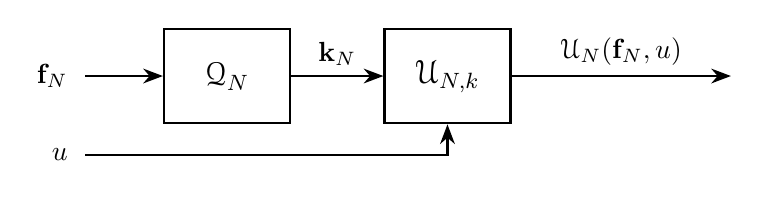
\begin{tikzpicture}[
    >={Stealth[length=2.5mm]},
    box/.style={draw, thick, minimum width=16mm, minimum height=12mm, font=\large},
    every node/.style={font=\normalsize},
]
\coordinate (fNin) at (0, 0.5);
\coordinate (uin)  at (0, -0.5);
\node[box] (QN) at (1.8, 0.5) {$\mathcal{Q}_N$};
\node[box] (UN) at (4.6, 0.5) {$\mathcal{U}_{N,k}$};
\coordinate (outR) at (8.2, 0.5);
\node[left=1mm of fNin] {$\mathbf{f}_N$};
\node[left=1mm of uin]  {$u$};
\draw[->, thick] (fNin) -- (QN.west);
\draw[->, thick] (QN.east) -- node[above] {$\mathbf{k}_N$} (UN.west);
\draw[->, thick] (uin) -- ++(4.6, 0) -- (UN.south);
\draw[->, thick] (UN.east) -- node[above] {$\mathcal{U}_N(\mathbf{f}_N, u)$} (outR);
\end{tikzpicture}%
}
\caption{Cascade of operators $\mathcal{Q}_N$ and $\mathcal{U}_{N,k}$ generates feedback control input $\mathcal{U}_N(\mathbf{f}_N, u)$.}
\label{fig:cascade}
\end{figure}

Two operations of different character connect $(\mathbf{f}_N, u)$ to $\mathcal{U}_N(\mathbf{f}_N, u)$ in Figure~\ref{fig:cascade}. The following theorem certifies that, jointly, they are Lipschitz.

\begin{theorem}[Joint Lipschitz property]
\label{thm:main}
Fix $N\ge 2$ and $B_f, L_f, R, L_u > 0$. The joint controller operator $\mathcal{U}_N$ defined in \eqref{eq:KNdef}, restricted to $\mathcal{U}_N \colon \mathcal{F}_N^\star(B_f,L_f) \times \mathcal{V}(R,L_u) \to \R$, satisfies
\begin{eqnarray}
\bigl|\mathcal{U}_N(\mathbf{f}_N,u) - \mathcal{U}_N(\tilde{\mathbf{f}}_N,\tilde u)\bigr| &\le& M_N(R)\,\|\mathbf{f}_N-\tilde{\mathbf{f}}_N\|_\star \nonumber \\
&& +\, M'_N(R)\,\|u-\tilde u\|_{\Linf(0,1)}
\label{eq:joint-Lip}
\end{eqnarray}
for all $\mathbf{f}_N,\tilde{\mathbf{f}}_N\in\mathcal{F}_N^\star(B_f,L_f)$ and all $u,\tilde u\in\mathcal{V}(R,L_u)$, where the operator Lipschitz constants are
\begin{equation}
M_N(R) := \sum_{n=2}^N \frac{R^n}{n!}\,\lambda_n, \quad M'_N(R) := \sum_{n=2}^N \frac{n R^{n-1}}{n!}\,\kappa_n,
\label{eq:M-def}
\end{equation}
with the kernel Lipschitz-in-$\mathbf{f}_N$ constants $\lambda_2 := 1$ and, for $3\le n\le N$,
\begin{equation}
\lambda_n := 1 + \sum_{m=2}^{n-1} \beta_{n,m}\bigl(B_f\,\lambda_{n-m+1} + \kappa_{n-m+1}\bigr),
\label{eq:lambda-def}
\end{equation}
the kernel sup-norm bounds $\kappa_2 := B_f$ and, for $3\le n\le N$,
\begin{equation}
\kappa_n := B_f + B_f\sum_{m=2}^{n-1} \beta_{n,m}\,\kappa_{n-m+1},
\label{eq:kappa-def}
\end{equation}
and the combinatorial constants
\begin{eqnarray}
\beta_{n,m} &:=& (n-m+1) \nonumber \\
&& \times\, \max_{1\le j\le n-m+1}\binom{n-j}{n-m+1-j} \nonumber \\
&\le& n\,2^n, \quad 2\le m\le n\le N.
\label{eq:beta-def}
\end{eqnarray}
In particular, $\mathcal{U}_N$ is locally Lipschitz on bounded sets in $\mathcal{F}_N^\star(B_f,L_f)\times\mathcal{V}(R,L_u)$.
\end{theorem}

The proof proceeds in two stages: first, that the kernels $k_n$ themselves are bounded and Lipschitz-continuous in $\mathbf{f}_N$ in sup-norm with constants $\kappa_n$ and $\lambda_n$ (Section~\ref{sec:knLip}); second, that the operator $\mathcal{U}_N(\mathbf{f}_N, u)$, as a multilinear functional, is Lipschitz in $(k_2, \ldots, k_N, u)$ (Section~\ref{sec:UNlip}). The two stages are then composed (Section~\ref{sec:proof}).

\begin{remark}
\label{rem:beta-bound}
The closed-form bound $\beta_{n,m}\le n\,2^n$ in \eqref{eq:beta-def} follows from $\binom{n-j}{n-m+1-j}\le 2^{n-j}\le 2^{n-1}$ and $n-m+1\le n$.
\end{remark}

\begin{remark}
\label{rem:kappa-growth}
The constants $\kappa_n, \lambda_n$, and hence $M_N(R), M'_N(R)$, grow super-exponentially in $N$, so the bound \eqref{eq:joint-Lip} is far from tight. It is not meant to be: the seminorms $L_f, L_u$ are absent from it entirely, serving only to render the input sets $\mathcal{F}_n(B_f,L_f)$ and $\mathcal{V}(R,L_u)$ compact in $\Linf$ (Arzel\`a--Ascoli). The bound is qualitative --- it certifies the continuity of $\mathcal{U}_N$ that the neural-operator universal approximation theorem of Section~\ref{sec:NO} requires.
\end{remark}

\section{Proof of Theorem~\ref{thm:main}}
\label{sec:proof-thm1}

\subsection{Sup-norm Bound on $B_n^m$}
\label{sec:Bbound}

All upper bounds on the kernels $k_n$ trace back to bounds on the bilinear blocks $B_n^m$ feeding the recursion. We start there.

\begin{lemma}[Bound on $B_n^m$]
\label{lem:Bbound}
For all $k\in\Linf(T_{n-m+1}(1))$, $f\in\Linf(T_m(1))$, and $2\le m\le n$,
\begin{eqnarray}
&& \|B_n^m[k,f]\|_{\Linf(\Delta_n)} \nonumber \\
&& \le\, \beta_{n,m}\,\|k\|_{\Linf(T_{n-m+1}(1))}\,\|f\|_{\Linf(T_m(1))},
\label{eq:Bbound}
\end{eqnarray}
with $\beta_{n,m}$ as in \eqref{eq:beta-def}.
\end{lemma}

\begin{proof}
For each $j\in\{1,\ldots,n-m+1\}$, the operator $D_j^{n-m+1,m}$ in \eqref{eq:Ddef} is, by definition, a sum over a set of cardinality $\binom{p+m-1-j}{p-j}$ with $p = n-m+1$, which equals $\binom{n-j}{n-m+1-j}$, of evaluations of $k$ at points of $T_{n-m+1}(1)$. Hence pointwise,
\begin{equation}
\bigl|\bigl[D_j^{n-m+1,m}k\bigr](\cdot)\bigr|
\le \binom{n-j}{n-m+1-j}\,\|k\|_{\Linf}.
\label{eq:Dbnd}
\end{equation}
The integral over $[\xi_j,\xi_{j-1}]\subseteq[0,1]$ contributes a factor at most $1$, and the outer summation is over $n-m+1$ values of $j$. Therefore, pointwise on $\Delta_n$,
\begin{eqnarray}
&& |B_n^m[k,f](\cdot)| \nonumber \\
&& \le (n-m+1)\,\max_{1\le j\le n-m+1}\binom{n-j}{n-m+1-j} \nonumber \\
&& \quad \times\, \|k\|_{\Linf}\,\|f\|_{\Linf} \nonumber \\
&& =\, \beta_{n,m}\,\|k\|_{\Linf}\,\|f\|_{\Linf}.
\label{eq:Bbnd-pw}
\end{eqnarray}
\end{proof}

\subsection{Lipschitz Dependence of $k_n$ on Plant Coefficients}
\label{sec:knLip}

We assemble the kernels generated from $\mathbf{f}_N$ via \eqref{eq:k2def}--\eqref{eq:kndef} into a tuple $\mathbf{k}_N = (k_2, \ldots, k_N)$, and write the kernel-generation recursion as the operator $\mathbf{k}_N = \mathcal{Q}_N(\mathbf{f}_N)$.
Lemma~\ref{lem:knBound} below establishes a sup-norm bound on $\mathcal{Q}_N$ on bounded sets, and Lemma~\ref{lem:knLip} establishes its Lipschitz continuity.

\begin{lemma}[Sup-norm bound for $k_n$]
\label{lem:knBound}
For every $\mathbf{f}_N\in\mathcal{F}_N^\star(B_f,L_f)$, the kernels $k_n$ defined by \eqref{eq:k2def}--\eqref{eq:kndef} satisfy
\begin{equation}
\|k_n\|_{\Linf(\Delta_n)} \le \kappa_n,
\qquad 2\le n\le N,
\label{eq:knBound}
\end{equation}
with $\kappa_n$ as in \eqref{eq:kappa-def}.
\end{lemma}

\begin{proof}
For $n=2$, \eqref{eq:k2def} gives, pointwise,
\begin{equation}
|k_2(x,\xi_1,\xi_2)| \le \int_0^{\xi_2} \|f_2\|_{\Linf}\,ds \le B_f,
\label{eq:k2-pw}
\end{equation}
since $\xi_2\in[0,1]$ and $\|f_2\|_{\Linf}\le B_f$. Hence $\|k_2\|_{\Linf}\le B_f = \kappa_2$.

For the inductive step, suppose \eqref{eq:knBound} holds for $2\le n'\le n-1$. From \eqref{eq:kndef}, pointwise on $\Delta_n$, $|k_n(x,\xi_1,\ldots,\xi_n)| \le \int_0^{\xi_n} [\|f_n\|_{\Linf} + \sum_{m=2}^{n-1} \|B_n^m[k_{n-m+1},f_m]\|_{\Linf}]\,ds$. Applying Lemma~\ref{lem:Bbound} and the inductive hypothesis $\|k_{n-m+1}\|_{\Linf}\le\kappa_{n-m+1}$, together with $\|f_m\|_{\Linf}\le B_f$,
\begin{eqnarray}
&& |k_n(x,\xi_1,\ldots,\xi_n)| \nonumber \\
&& \le \int_0^{\xi_n}\Bigl[B_f + B_f\sum_{m=2}^{n-1} \beta_{n,m}\,\kappa_{n-m+1}\Bigr]\,ds \nonumber \\
&& \le B_f + B_f\sum_{m=2}^{n-1} \beta_{n,m}\,\kappa_{n-m+1}
\;=\; \kappa_n,
\label{eq:kn-pw-2}
\end{eqnarray}
using $\xi_n\in[0,1]$ and \eqref{eq:kappa-def}.
\end{proof}

Lemma~\ref{lem:knBound} controls the size of each $k_n$. We now control how $k_n$ moves when the plant coefficients $\mathbf{f}_N$ are perturbed.

\begin{lemma}[Lipschitz dependence of $k_n$]
\label{lem:knLip}
For every $\mathbf{f}_N,\tilde{\mathbf{f}}_N\in\mathcal{F}_N^\star(B_f,L_f)$, with $k_n,\tilde k_n$ the corresponding kernels defined by \eqref{eq:k2def}--\eqref{eq:kndef},
\begin{equation}
\|k_n - \tilde k_n\|_{\Linf(\Delta_n)}
\le \lambda_n\,\|\mathbf{f}_N-\tilde{\mathbf{f}}_N\|_\star,
\label{eq:knLip}
\end{equation}
for $2\le n\le N$, with $\lambda_n$ as in \eqref{eq:lambda-def}.
\end{lemma}

\begin{proof}
For $n=2$, subtract \eqref{eq:k2def} for $\tilde f_2$ from that for $f_2$, and bound pointwise:
\begin{eqnarray}
&& |k_2(x,\xi_1,\xi_2) - \tilde k_2(x,\xi_1,\xi_2)| \nonumber \\
&& \le \int_0^{\xi_2} \|f_2 - \tilde f_2\|_{\Linf}\,ds \nonumber \\
&& \le \|f_2 - \tilde f_2\|_{\Linf}
\;\le\; \|\mathbf{f}_N-\tilde{\mathbf{f}}_N\|_\star,
\label{eq:k2diff-pw}
\end{eqnarray}
so \eqref{eq:knLip} holds with $\lambda_2 = 1$.

For the inductive step, suppose \eqref{eq:knLip} holds for $2\le n'\le n-1$. The bilinearity of $B_n^m$ in its two arguments gives the splitting
\begin{eqnarray}
&& B_n^m[k_{n-m+1},f_m] - B_n^m[\tilde k_{n-m+1},\tilde f_m] \nonumber \\
&& = B_n^m[k_{n-m+1}-\tilde k_{n-m+1},\,f_m] \nonumber \\
&& \quad +\, B_n^m[\tilde k_{n-m+1},\,f_m - \tilde f_m].
\label{eq:B-bilinear-split}
\end{eqnarray}
Applying Lemma~\ref{lem:Bbound} to each term, and using $\|k_{n-m+1}-\tilde k_{n-m+1}\|_{\Linf}\le \lambda_{n-m+1}\|\mathbf{f}_N-\tilde{\mathbf{f}}_N\|_\star$ (inductive hypothesis), $\|f_m\|_{\Linf}\le B_f$, $\|\tilde k_{n-m+1}\|_{\Linf}\le\kappa_{n-m+1}$ (Lemma~\ref{lem:knBound}), and $\|f_m-\tilde f_m\|_{\Linf}\le\|\mathbf{f}_N-\tilde{\mathbf{f}}_N\|_\star$,
\begin{eqnarray}
&& \|B_n^m[k_{n-m+1},f_m] - B_n^m[\tilde k_{n-m+1},\tilde f_m]\|_{\Linf} \nonumber \\
&& \le \beta_{n,m}\bigl(B_f\,\lambda_{n-m+1} + \kappa_{n-m+1}\bigr) \nonumber \\
&& \quad \times\, \|\mathbf{f}_N-\tilde{\mathbf{f}}_N\|_\star.
\label{eq:Bdiff-bnd}
\end{eqnarray}
Subtracting the $\tilde{\mathbf{f}}_N$ version of \eqref{eq:kndef} from the $\mathbf{f}_N$ version and applying these bounds termwise,
\begin{eqnarray}
|k_n - \tilde k_n| &\le& \int_0^{\xi_n}\Bigl[\|\mathbf{f}_N-\tilde{\mathbf{f}}_N\|_\star + \sum_{m=2}^{n-1} \beta_{n,m} \nonumber \\
&& \times\bigl(B_f\,\lambda_{n-m+1} + \kappa_{n-m+1}\bigr) \nonumber \\
&& \times\, \|\mathbf{f}_N-\tilde{\mathbf{f}}_N\|_\star\Bigr]\,ds \nonumber \\
&\le& \lambda_n\,\|\mathbf{f}_N-\tilde{\mathbf{f}}_N\|_\star,
\label{eq:kndiff-pw}
\end{eqnarray}
using $\xi_n\le 1$ and \eqref{eq:lambda-def}.
\end{proof}

\subsection{Lipschitz Dependence of $\mathcal{U}_N(\mathbf{f}_N, u)$ on $(\mathbf{k}_N, u)$}
\label{sec:UNlip}

The operator $\mathcal{U}_{N,k}$ in \eqref{eq:KNdef} is a sum of $n$-fold integrals $J_n$ over $n = 2, \ldots, N$. We bound each $J_n$ separately, then sum.

\begin{lemma}[Multilinear bound]
\label{lem:single-order}
Fix $n\in\{2,\ldots,N\}$ and define
\begin{equation}
J_n[k,u] := \int_{T_n(1)} k(\xi_1,\ldots,\xi_n)\,\prod_{i=1}^n u(\xi_i)\,d\xi_n\cdots d\xi_1,
\label{eq:Jdef}
\end{equation}
for $k\in\Linf(T_n(1))$ and $u\in\Linf(0,1)$. Then for $\|k\|_{\Linf},\|\tilde k\|_{\Linf}\le K$ and $\|u\|_{\Linf},\|\tilde u\|_{\Linf}\le R$,
\begin{eqnarray}
&& |J_n[k,u] - J_n[\tilde k,\tilde u]| \nonumber \\
&& \le \frac{R^n}{n!}\,\|k-\tilde k\|_{\Linf}
+ \frac{K\,n R^{n-1}}{n!}\,\|u-\tilde u\|_{\Linf}.
\label{eq:JLip}
\end{eqnarray}
\end{lemma}

\begin{proof}
The simplex volume is $|T_n(1)| = 1/n!$. Write
\begin{eqnarray}
&& J_n[k,u] - J_n[\tilde k,\tilde u] \nonumber \\
&& = J_n[k-\tilde k,u] + J_n[\tilde k,\,u^{\otimes n} - \tilde u^{\otimes n}],
\label{eq:Jdiff-split}
\end{eqnarray}
where $u^{\otimes n}(\xi) := \prod_i u(\xi_i)$ and similarly for $\tilde u$. The first term satisfies $|J_n[k-\tilde k,u]| \le \|k-\tilde k\|_{\Linf}\,R^n / n!$. For the second, the multilinear telescoping identity
\begin{eqnarray}
\prod_{i=1}^n u(\xi_i) - \prod_{i=1}^n \tilde u(\xi_i) &=& \sum_{j=1}^n \Bigl[\prod_{i<j} u(\xi_i)\Bigr]\bigl(u(\xi_j) - \tilde u(\xi_j)\bigr) \nonumber \\
&& \times\, \Bigl[\prod_{i>j}\tilde u(\xi_i)\Bigr]
\label{eq:telescope}
\end{eqnarray}
yields, on $T_n(1)$ with $\|u\|_{\Linf},\|\tilde u\|_{\Linf}\le R$,
\begin{equation}
\bigl|u^{\otimes n}(\xi) - \tilde u^{\otimes n}(\xi)\bigr|
\le n R^{n-1}\,\|u-\tilde u\|_{\Linf},
\label{eq:tensor-diff}
\end{equation}
hence $|J_n[\tilde k,\,u^{\otimes n} - \tilde u^{\otimes n}]| \le K\,n R^{n-1}\,\|u-\tilde u\|_{\Linf} / n!$. Adding gives \eqref{eq:JLip}.
\end{proof}

\subsection{Completing the proof of Theorem~\ref{thm:main}}
\label{sec:proof}

Fix $\mathbf{f}_N,\tilde{\mathbf{f}}_N\in\mathcal{F}_N^\star(B_f,L_f)$ and $u,\tilde u\in\mathcal{V}(R,L_u)$, and let $k_n,\tilde k_n$ be the kernels generated from $\mathbf{f}_N$ and $\tilde{\mathbf{f}}_N$ via \eqref{eq:k2def}--\eqref{eq:kndef}. By Lemma~\ref{lem:knBound}, $\|k_n\|_{\Linf(\Delta_n)},\|\tilde k_n\|_{\Linf(\Delta_n)}\le\kappa_n$ for $2\le n\le N$. By Lemma~\ref{lem:knLip}, $\|k_n-\tilde k_n\|_{\Linf(\Delta_n)}\le\lambda_n\,\|\mathbf{f}_N-\tilde{\mathbf{f}}_N\|_\star$. Since the boundary traces $k_n(1,\cdot)$ are restrictions of $k_n$ to the slice $\{x = 1\}$ of $\Delta_n$, the same bounds hold with $\Linf(T_n(1))$ in place of $\Linf(\Delta_n)$.

Applying Lemma~\ref{lem:single-order} to each summand of \eqref{eq:KNdef} with $K=\kappa_n$,
\begin{eqnarray}
|\mathcal{U}_N(\mathbf{f}_N,u) - \mathcal{U}_N(\tilde{\mathbf{f}}_N,\tilde u)| &\le& \sum_{n=2}^N\Bigl[\frac{R^n}{n!}\,\|k_n-\tilde k_n\|_{\Linf} \nonumber \\
&& +\, \frac{\kappa_n\,n R^{n-1}}{n!}\,\|u-\tilde u\|_{\Linf}\Bigr].
\label{eq:UN-diff-bnd}
\end{eqnarray}
Substituting $\|k_n-\tilde k_n\|_{\Linf}\le\lambda_n\,\|\mathbf{f}_N-\tilde{\mathbf{f}}_N\|_\star$ and using \eqref{eq:M-def} yields \eqref{eq:joint-Lip}. Local Lipschitz continuity on bounded sets is immediate.


\section{Neural Operator Approximation}
\label{sec:NO}

\begin{figure*}[t]
\centering
\resizebox{0.81\linewidth}{!}{%
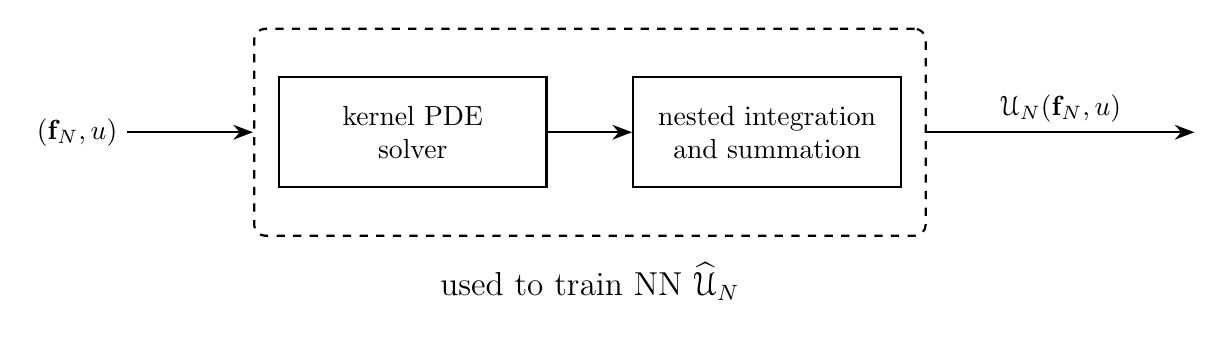
\begin{tikzpicture}[
    >={Stealth[length=2.5mm]},
    innerbox/.style={draw, thick, minimum width=34mm, minimum height=14mm, font=\normalsize, align=center},
    every node/.style={font=\normalsize},
]
\node[innerbox] (PDE) at (3.0, 0) {kernel PDE\\ solver};
\node[innerbox] (NI)  at (7.5, 0) {nested integration\\ and summation};
\draw[->, thick] (PDE.east) -- (NI.west);
\begin{pgfonlayer}{background}
  \node[draw, dashed, thick, rounded corners,
        inner xsep=3mm, inner ysep=6mm,
        fit=(PDE)(NI)] (NN) {};
\end{pgfonlayer}
\coordinate (inAnchor) at ($(NN.west) + (-1.6, 0)$);
\node[left=0pt of inAnchor] (in) {$(\mathbf{f}_N, u)$};
\coordinate (outAnchor) at ($(NN.east) + (3.4, 0)$);
\draw[->, thick] (in.east) -- (NN.west);
\draw[->, thick] (NN.east) -- node[above] {$\mathcal{U}_N(\mathbf{f}_N, u)$} (outAnchor);
\node[below=2mm of NN.south, font=\large] {used to train NN $\widehat{\mathcal{U}}_N$};
\end{tikzpicture}%
}
\caption{Neural operator $\widehat{\mathcal{U}}_N$ subsumes the cascade of Figure~\ref{fig:cascade} --- kernel PDE solution and nested integration --- into a single trained mapping from $(\mathbf{f}_N, u)$ to $\mathcal{U}_N(\mathbf{f}_N, u)$.}
\label{fig:NO-cascade}
\end{figure*}

The neural-operator universal approximation theorem~\cite{Lu2021Universal}, applied to operators continuous on compact sets, ensures the existence of a neural-operator surrogate $\widehat{\mathcal{U}}_N$ for $\mathcal{U}_N$ within any prescribed accuracy (Figure~\ref{fig:NO-cascade}).


\begin{theorem}[Neural-operator surrogate]
\label{thm:NO}
For every $\eps > 0$, there exists a neural operator $\widehat{\mathcal{U}}_N : \mathcal{F}_N^\star(B_f,L_f) \times \mathcal{V}(R,L_u) \to \R$ such that
\begin{eqnarray}
&& \bigl|\mathcal{U}_N(\mathbf{f}_N, u) - \widehat{\mathcal{U}}_N(\mathbf{f}_N, u)\bigr| \le \eps, \nonumber \\
&& \forall\,(\mathbf{f}_N, u) \in \mathcal{F}_N^\star(B_f,L_f) \times \mathcal{V}(R,L_u).
\label{eq:NObnd}
\end{eqnarray}
\end{theorem}

\begin{proof}
By Theorem~\ref{thm:main}, $\mathcal{U}_N$ is Lipschitz on $\mathcal{F}_N^\star(B_f,L_f)\times\mathcal{V}(R,L_u)$, hence continuous; the input set is compact in $\Linf$ by Arzel\`a--Ascoli. The result then follows from the universal approximation theorem of~\cite{Lu2021Universal}.
\end{proof}


\begin{thebibliography}{99}
\bibitem[]{Lu2021Universal} Lu, Lu; Jin, Pengzhan; Pang, Guofei; Zhang, Zhongqiang; Karniadakis, George Em. Learning nonlinear operators via {DeepONet} based on the universal approximation theorem of operators. Nature Machine Intelligence 3 (2021) 218--229
\bibitem[]{krstic2026feedbacklinearizationhyperbolicpdes} Miroslav Krstic. Feedback Linearization of Hyperbolic PDEs with Volterra Nonlinearities. (2026)
\bibitem[]{krstic2026feedbacklinearizationhyperbolicpdes-trunc} Krstic, Miroslav. Approximate Feedback Linearization for a Nonlinear Hyperbolic {PDE} Class --- {Part I}: {Volterra} Truncation. (2026)
\end{thebibliography}
\end{document}
